\documentclass[11pt,a4paper]{article}

\usepackage[margin=1in]{geometry}
\usepackage{amsmath}
\usepackage{amssymb}
\usepackage{amsthm}
\usepackage{booktabs}
\usepackage{graphicx}
\usepackage{tikz}
\usepackage[hidelinks,unicode]{hyperref}

\hypersetup{
  pdftitle={Certified Split Points: Parallel Lexing Without Speculation},
  pdfauthor={Nicklas Nidhögg},
  pdfsubject={Parallel lexical analysis; deterministic finite automata; maximal munch tokenization},
  pdfkeywords={parallel lexing, tokenization, deterministic finite automata, maximal munch, split points}
}

\theoremstyle{definition}
\newtheorem{definition}{Definition}

\theoremstyle{plain}
\newtheorem{lemma}{Lemma}
\newtheorem{theorem}{Theorem}
\newtheorem{corollary}{Corollary}
\newtheorem{proposition}{Proposition}

\newcommand{\code}[1]{\texttt{#1}}

% The default itemize bullet pulls in a Type 3 bitmap font, which some submission systems reject. The math bullet
% comes from the Type 1 symbol font that is embedded already.
\renewcommand{\labelitemi}{\(\bullet\)}

\title{Certified Split Points:\\Parallel Lexing Without Speculation}
\author{Nicklas Nidh\"ogg\\[0.4em] \normalsize Independent Researcher\\ \normalsize
\texttt{nicklas.nidhogg@gmail.com}\\ \normalsize ORCID: 0009-0006-6161-6150}
\date{July 2026}

\begin{document}

\maketitle

\begin{abstract}
Table-driven DFA lexing is sequential: each transition depends on the state the previous byte produced. Scanning one
input in parallel therefore needs each chunk's entry state, which existing methods recover by simulating from every
state, by speculating and repairing, by prescanning, or by overlapping and verifying. We give a condition under which
no recovery is needed. For a longest-match scanner that restarts from $q_0$ at every token boundary, a byte $b$ is a
\emph{certified split symbol} when no state other than $q_0$ has a $b$-transition whose target can reach acceptance,
and $q_0$ is not re-entrant if it has one. Every occurrence of a certified byte in a completely tokenizable input
begins a token, so chunks starting there reproduce the serial sequence of token kinds and lengths by ordered
concatenation, with no speculation, no overlap, and no merge beyond it. The condition is necessary as well as
sufficient, so a token set certifying nothing admits no single-byte split symbol at all. Deriving it costs
$O(|Q|\,|\Sigma|)$ once and leaves the scan loop untouched. Implemented in the munch lexer library~\cite{munch}, it
reaches 93--95\% parallel efficiency at eight threads on a 512\,MiB corpus four times the last-level cache, and a
$3.5$--$3.9\times$ end-to-end speedup at four threads, both across two benchmark revisions on one machine. The method
is deliberately partial, since one string,
comment, or run token can eliminate every useful certificate; it turns delimiter-based parallel lexing from a
language-specific assumption into a property a compiler checks.
\end{abstract}

\section{Introduction}

A table-compiled scanner executes, per input byte, one transition of the form
\[
  \code{state = table[row(byte) + state]}.
\]
The load producing the next state cannot begin before the previous state is known, so the scan is a serial
dependency chain whose throughput is bounded by the load-to-use latency of the cache holding the table. Once an
implementation reaches that floor, further speedup on a single input must come from scanning several regions of it
at once.

Splitting is the obstacle. A scanner dropped at an arbitrary offset does not know the automaton state there: the offset
may fall inside a string literal, halfway through an identifier, or in the middle of a multi-byte operator. A
tokenization computed from a wrong entry state is wrong until the scanner happens to resynchronize, and whether and when
it resynchronizes depends on both the automaton and the input.

This report describes a property that removes the uncertainty for a useful class of token sets, rather than managing it.
The property is a per-symbol certificate, extracted from the compiled automaton at construction time, that identifies
bytes which cannot occur strictly inside a token. Chunk boundaries placed immediately before such bytes need no
speculation and no reconciliation: the concatenated per-chunk token streams are exactly the serial stream.

\begin{samepage}
The contributions are:

\begin{itemize}
\item a static condition on a compiled token automaton identifying the bytes at which a longest-match scanner is
      provably between tokens, including the re-entrancy requirement without which the natural criterion is unsound
      (Section~\ref{sec:certificate});
\item a proof that the condition is not only sufficient but necessary, once transitions that can never reach
      acceptance are excluded, so that a token set certifying nothing admits no single-byte split symbol at all
      (Section~\ref{sec:necessity});
\item a linear-time derivation, a boundary planner, and an exactness theorem for the resulting parallel scan,
      implemented and released in a general-purpose lexer library (Sections~\ref{sec:derivation}
      and~\ref{sec:evaluation});
\item a survey of token sets showing where the property holds and where a single token kind destroys it, which
      grounds the folklore that source text can be split at line boundaries (Section~\ref{sec:applicability}).
\end{itemize}
\end{samepage}

Section~\ref{sec:prior} places the certificate among the existing answers to the entry-state problem, and
Section~\ref{sec:evaluation} reports what it costs and what it buys.

\section{Prior approaches}
\label{sec:prior}

Published solutions accept the unknown-state problem and manage it.

\paragraph{Compile the simulation into the automaton.} Simultaneous finite automata~\cite{sinya2013sfa} take a
state of the extended automaton to be a mapping from entry state to exit state, so one ordinary pass over a chunk
yields that chunk's whole transfer function; the mappings compose associatively and chunks combine in a parallel
reduction. The per-state simulation is therefore paid at construction rather than at scan time, and the authors
report almost no runtime overhead. What it costs is the size of the constructed automaton: a state is a map on states,
so the worst case is $n^n$ from a DFA with $n$ states and $2^{n^2}$ from an NFA, though for the expressions they
survey it is usually far smaller: of the more than 20,000 SNORT expressions they measure, 98.6\% give a D-SFA no
larger than the square of the minimal DFA, 279 exceed it and six exceed its cube. The reduction step also remains.
Composition can also be applied directly instead of compiled in, and in that form it is the oldest answer of all:
Hillis and Steele~\cite{hillis1986dataparallel} treat each character as a unary function on states, observe that the
induced composition is associative, and recover the state after every character with one parallel-prefix operation.
Their worked example is lexing program text. Data-parallel finite-state machines~\cite{mytkowicz2014dpfsm} take the
same route on SIMD and multicore hardware, enumerating transitions from every possible start state so that the
enumeration is exactly the transition function, and citing Hillis and Steele as the basis for doing so; the correct
computation is selected afterwards, so nothing is guessed and nothing needs repair. The cost is a factor of $|Q|$ in
work, which convergence reduces in practice, though the authors report that convergence to a single state is rare. A
GPU lexer applies the same scan to recover the complete state stream, the state after every input position rather than
only each chunk's entry state~\cite{voetter2021gpu}. Holding one function table per input position costs $O(|Q|n)$
space, so that work precomputes the reachable compositions and identifies each by an integer, reducing composition to
a two-dimensional lookup. The trade is the same one the simultaneous construction makes, paid in a table rather than
in states.

\paragraph{Carry fewer entry states.} Composition is exact but pays for every state. A second family attacks that cost
by shrinking the set a chunk must carry. Enumerative speculation sits deliberately between the extremes: rather than
speculating on a single state or enumerating all of them, it speculates transitions from several states chosen by a
lookback over the preceding input~\cite{jiang2017enumerative}. Reduced-interface DFAs~\cite{borsotti2025ridfa} attack
the same overhead from the automaton side, cutting the number of starting states a chunk automaton must carry by
combining an NFA's state reduction with deterministic transitions. What remains uncertain in this family is how much
redundant work is left when a speculation misses, and with it the speedup.

\paragraph{Relocate cuts to a language's separators.} Parallel lexers have long been built by cutting near equal
divisions and sliding each cut to a language-specific separator~\cite{barenghi2015parallel}. The separator and the
search bound are chosen by hand, and finding a separator does not by itself remove the entry-state problem: the
accompanying parallel lexical analysis enumerates the possible start states of a chunk rather than deducing one, with
each worker carrying one computation per alternative and up to four at once in the worst
case~\cite{barenghi2015parallel}. The technique is therefore separator relocation combined with state enumeration, not a
proof that the separator is safe. Its worked cases are the direct antecedent of
Section~\ref{sec:applicability}: newline preserves JSON's non-trivia token stream, since no non-trivia lexeme admits
it, yet it is rejected in practice because generated JSON may contain none. Lua fails for a stronger reason than any
certificate could address: its long-bracket delimiters \code{[=$^n$[} and \code{]=$^n$]} must agree on $n$, so the
lexical grammar is not regular, the set of possible delimiters is unbounded, and with it the set of possible entry
states; no fixed lookahead can decide which delimiter, if any, encloses a chunk~\cite{barenghi2015parallel}. Barenghi
et al. recover a workable schema only by constraining the language, admitting just \code{[[} and \code{]]} for strings
and requiring multi-line comments to end at a newline, after which newline does serve as their split point. What is
missing is any way to decide, from the token set alone, whether a proposed separator is sound.

\paragraph{Prescan for context.} Plex~\cite{li2021plex} removes the need for delimiters entirely. It derives a
prescanning automaton from the lexer's own DFA, embedding backtracking cases into it, and runs that automaton over
the input to compute a transfer function per chunk; composing the transfer functions yields each chunk's true entry
state, after which chunks scan in parallel with no language-specific analysis. The price is a pass over the input;
the benefit is that it applies to grammars that certify nothing here.

\paragraph{Analyse the grammar for streaming.} StreamTok~\cite{li2026streaming} is the closest methodological
neighbour: it also analyses a maximal-munch token grammar statically, before any input, and also partitions
grammars into those its technique serves and those it does not. What it computes is different. Its maximum token
neighbour distance bounds how far a longest-match decision can depend on future input, which is what makes
bounded-memory streaming possible; it derives no separators and claims no boundaries, and parallelising it is left
as future work there. The two analyses are complementary: StreamTok bounds the context needed to confirm a token,
the certificate identifies positions where no preceding context is needed at all.

\paragraph{Recover a restart point after an edit.} Incremental lexers face the mirror of this
question~\cite{wagner1997lexing}: after an edit, how far back must re-lexing begin for the result to equal a full
re-scan. They answer it dynamically and per edit, saving the batch machine's state with each token as it is created
so analysis can restart at any token boundary, and tracking lookahead dependencies as they arise rather than bounding
them in advance. The certificate answers a static question instead, once per token set and before any input exists,
and the two are complementary: a restart point is a fact about one input and its history, a certified byte is a
fact about the grammar. An incremental divide-and-conquer lexer~\cite{hugo2015incremental} takes the other route
open to it, storing a result for every possible entry state of a fragment and composing the resulting transition
maps, which places it with the all-state family rather than with boundary certification.

\paragraph{Restrict the automaton.} Holub and \v{S}tekr's parallel run~\cite{holub2009parallel} is exact and
efficient for $k$-local automata, in which any $k$ consecutive symbols force a unique state regardless of the
starting state. The property is uniform over the whole automaton rather than per symbol, and a lexical grammar need
not have it.

\paragraph{Realign after the fact.} Parallel tokenization for language-model vocabularies faces the same boundary
problem, and the overlap-based answer to it, extending chunks so neighbours share a region and merging inside it, does
not guarantee the sequential result. LoPT~\cite{shao2026lopt} instead matches on character positions and adjusts chunk
lengths dynamically to realign the segments, and proves the merged output identical to sequential tokenization.

\paragraph{Assume a delimiter.} Data systems split logs and CSV at newlines because ``records do not contain
newlines'', adjusting each cut to the next delimiter. The assumption is per-format and informal, and it is famously
unsound for CSV with quoted newlines, which is why speculative CSV parsing is a research topic~\cite{ge2019csv};
massively parallel delimiter parsing~\cite{stehle2020parparaw} attacks the same context problem on GPUs.
Format-specific structural scans~\cite{li2017mison,langdale2019simdjson,cameron2008parabix} hand-derive comparable
facts per format.

None of these asks the token set's own automaton which bytes are safe.

\section{Preliminaries}
\label{sec:prelim}

Let $\Sigma$ be the byte alphabet. We take a compiled token set to be a deterministic automaton $A = (Q, \Sigma, \delta,
q_0, \tau)$ with a partial transition function $\delta : Q \times \Sigma \rightharpoonup Q$, an initial state $q_0 \in
Q$, and a partial accepting map $\tau : Q \rightharpoonup T$ assigning a token to accepting states. We write
$\delta^*(q, u)$ for the state reached from $q$ on $u \in \Sigma^*$ when every transition along the way is defined, and
say $\delta^*(q,u)$ is undefined otherwise.

The scanner is the usual longest-match loop. At offset $i$ of an input $w \in \Sigma^*$ it starts in $q_0$, consumes
bytes while transitions are defined, remembers the last position at which $\tau$ was defined, emits the token found
there, and restarts at that position in $q_0$. If no accepting position is reached, the scan halts at $i$. Tokens are
positive-length: acceptance counts only after at least one symbol has been consumed, so an accepting $q_0$ never emits
the empty word and the loop always advances. Without that rule the loop is undefined exactly where
Section~\ref{sec:subtlety} needs it, since a nullable token set accepts at $i$ after zero bytes and would restart at $i$
forever. The batch and parallel entry points of the implementation enforce the rule, treating a zero-length acceptance
as no match and halting at the offset; the single-match entry point returns the length-zero match instead, and a caller
looping over it must reject that itself. The composite system is therefore not a single automaton run: it is a run that
\emph{resets to $q_0$ at every token boundary}, and the certificate exploits exactly that reset.

Write $\mathrm{tok}(w)$ for the sequence of (token, length) pairs the scanner emits on $w$, and $\mathrm{con}(w)$ for
the number of bytes it consumes. Call $w$ \emph{completely tokenizable} when $\mathrm{con}(w) = |w|$, and call an offset
$i$ a \emph{token boundary} of $w$ when the scanner starts a token at $i$ (with $|w|$ itself a boundary).

\section{The certificate}
\label{sec:certificate}

Only transitions that can still end in acceptance can lie on an emitted token, and the certificate is defined over
those alone. Write
\[
  Q^+ = \{\, q \in Q \mid \delta^*(q, v) \text{ is accepting for some } v \in \Sigma^* \,\}
\]
for the co-accessible states, and let $\delta^+(q, a) = \delta(q, a)$ when that transition is defined and
$\delta(q, a) \in Q^+$, and be undefined otherwise. All that follows is stated over the \emph{live subautomaton}
$A^+ = (Q^+, \Sigma, \delta^+, q_0, \tau)$. Section~\ref{sec:necessity} shows why the restriction is not cosmetic:
a pattern denoting the empty language leaves states in $Q \setminus Q^+$ whose transitions would otherwise
de-certify symbols that no token can contain. If $q_0 \notin Q^+$ the token set accepts nothing, and no symbol is
useful; we assume $q_0 \in Q^+$ throughout. One consequence is used repeatedly below: the match path of any emitted
token lies in $A^+$ throughout, since every transition along it leads to that token's accepting position, so
reasoning about emitted tokens may read $\delta$ as $\delta^+$ without further comment.

\begin{definition}[Re-entrant initial state]
\label{def:reentrant}
$q_0$ is \emph{re-entrant} if $(\delta^+)^*(q_0, u) = q_0$ for some $u \in \Sigma^+$.
\end{definition}

Because every state of a compiled automaton is reachable, Definition~\ref{def:reentrant} is equivalent to $q_0$ having
an incoming live transition, which is how an implementation tests it.

\begin{definition}[Certified split symbol]
\label{def:certified}
A symbol $b \in \Sigma$ is \emph{certified} if every $q \in Q^+$ with $\delta^+(q, b)$ defined satisfies $q = q_0$,
and if $\delta^+(q_0, b)$ is defined then $q_0$ is not re-entrant.
\end{definition}

The exemption for $q_0$ is what makes the definition useful rather than vacuous: a token may legitimately begin with
$b$. The exemption is sound only while no input can return the automaton to $q_0$ mid-scan, which is precisely the
re-entrancy condition. Section~\ref{sec:subtlety} shows that dropping it makes the certificate false.

\begin{lemma}[Occurrences begin tokens]
\label{lem:boundary}
Let $b$ be certified and let $w$ be completely tokenizable. Then every offset of $w$ holding $b$ is a token boundary
of $w$.
\end{lemma}

\begin{proof}
Let $w_i = b$ and suppose $i$ is not a token boundary. Since $w$ is completely tokenizable, every offset is either a
token boundary or lies strictly inside some emitted token, so $i$ lies strictly inside a token that starts at some
$s < i$. Let $u = w_s \cdots w_{i-1}$, which is nonempty, and let $q = (\delta^+)^*(q_0, u)$, the state immediately
before $b$ is consumed. The token's match path continues through offset $i$, so $\delta^+(q, b)$ is defined. By
Definition~\ref{def:certified}, $q = q_0$, hence $(\delta^+)^*(q_0, u) = q_0$ with $u$ nonempty, so $q_0$ is re-entrant
by Definition~\ref{def:reentrant}. But $\delta^+(q_0, b) = \delta^+(q, b)$ is defined, so Definition~\ref{def:certified}
also requires $q_0$ not to be re-entrant, a contradiction.
\end{proof}

\begin{theorem}[Split invariance]
\label{thm:main}
Let $w$ be completely tokenizable and let $0 = c_0 < c_1 < \cdots < c_m = |w|$ be offsets such that each interior
$c_j$ holds a certified symbol. Then
\[
  \mathrm{tok}(w) \;=\; \mathrm{tok}(w_{[c_0,c_1)}) \cdot \mathrm{tok}(w_{[c_1,c_2)}) \cdots
  \mathrm{tok}(w_{[c_{m-1},c_m)}),
\]
where $\cdot$ denotes concatenation of token sequences and $w_{[a,b)}$ the corresponding slice.
\end{theorem}

\begin{proof}
By Lemma~\ref{lem:boundary} every interior $c_j$ is a token boundary of $w$, and $c_0$ and $c_m$ are boundaries
trivially. Two facts are then needed. First, the scanner is deterministic and enters each token in state $q_0$ with no
state carried across boundaries, so a scan started at $c_j$ begins exactly as the global scan does there. Second,
while matching the last token of the chunk the global scan records no accepting position beyond $c_{j+1}$. Let
$q$ be the state reached on the nonempty prefix ending just before $c_{j+1}$. If $\delta^+(q, b)$ were defined for the
certified $b$ at $c_{j+1}$, the argument of Lemma~\ref{lem:boundary} would force $q = q_0$ and make $q_0$ re-entrant,
which Definition~\ref{def:certified} forbids; so it is not. Either $\delta(q, b)$ is undefined, and the scan stops at
$c_{j+1}$, or its target lies outside $Q^+$: were it inside, $q$ would itself be co-accessible and $\delta^+(q, b)$
would be defined. In the second case the scan may read on but can never reach an accepting state again. Note that the
scan is therefore not required to \emph{stop} at $c_{j+1}$, only to find nothing past it: lookahead may cross the
boundary through transitions that lead nowhere. Either way the last accepting position it recorded lies at or before
$c_{j+1}$, and the chunk scan, seeing the same bytes from the same state, records the same one, so the tokens emitted
between $c_j$ and $c_{j+1}$ coincide. Induction over $j$ gives the claim.
\end{proof}

\begin{lemma}[Boundaries before the first failure]
\label{lem:prefix}
Let $b$ be certified and let $w$ be any input. Every offset $i < \mathrm{con}(w)$ with $w_i = b$ is a token boundary
of the serial scan of $w$.
\end{lemma}

\begin{proof}
Every offset below $\mathrm{con}(w)$ is either a token boundary or lies strictly inside a token the scan emitted, so
if $i$ is not a boundary it lies strictly inside a token starting at some $s < i$. The argument of
Lemma~\ref{lem:boundary} applies unchanged to that token: the state $q$ reached on the nonempty $w_s \cdots w_{i-1}$
has $\delta^+(q,b)$ defined, hence $q = q_0$ by Definition~\ref{def:certified}, hence $q_0$ is re-entrant, which
Definition~\ref{def:certified} forbids once $\delta^+(q_0,b)$ is defined. Completeness of the tokenization is never
used, only that the offsets below $\mathrm{con}(w)$ were successfully traversed.
\end{proof}

\begin{corollary}[Malformed input] \label{cor:malformed} If $\mathrm{con}(w) < |w|$, let $[c_j, c_{j+1})$ be the chunk
containing the first failure. By Lemma~\ref{lem:prefix} every interior boundary below $\mathrm{con}(w)$ is a token
boundary of the serial scan, so the reasoning of Theorem~\ref{thm:main} applies to the chunks before it. Every
chunk before $c_j$ is fully consumed and contributes exactly the tokens the serial
scan emits there, and the chunk containing the failure halts at the same offset. The serial stream is therefore a
prefix of the concatenation, but chunks after the failure may emit tokens the serial scan never reaches. A caller must
check every chunk's consumed length before treating the concatenation as a successful tokenization. \end{corollary}

\begin{proposition}[Vacuous certificates]
\label{prop:vacuous}
If no $q \in Q^+$ has $\delta^+(q,b)$ defined, then $b$ is certified, and no completely tokenizable input contains $b$.
\end{proposition}

\begin{proof}
The first claim holds because Definition~\ref{def:certified} quantifies over an empty set. For the second, a
completely tokenizable $w$ containing $b$ would have $b$ consumed by some emitted token, whose match path lies in
$A^+$, so some state of $Q^+$ would consume $b$ live.
\end{proof}

Such symbols are certified but useless for planning: they cannot appear in valid input. They are also separable
mechanically, with no further analysis. If $b$ is certified then every live state consuming it is $q_0$, so $b$ is
consumed live by some state exactly when $\delta^+(q_0, b)$ is defined:

\begin{corollary}[Useful certificates]
\label{cor:useful}
A certified $b$ is non-vacuous if and only if $\delta^+(q_0, b)$ is defined.
\end{corollary}

An implementation can therefore report the useful set with no extra analysis, by intersecting the certificate with the
initial state's live transitions, which is what the predicate in the accompanying library reports: vacuous certificates
never reach a caller, since a caller cannot act on one and a planner searching for one scans the whole input for
nothing.

\subsection{The condition is also necessary}
\label{sec:necessity}

Definition~\ref{def:certified} is stated as a test, and Lemma~\ref{lem:boundary} shows it is sufficient. It is also
necessary, so nothing is given away by using it. Every state of $Q^+$ is co-accessible by construction, and every state
of a compiled automaton is reachable because subset construction discovers only reachable subsets, so the theorem
applies to every compiled token set.

\begin{theorem}[Characterization]
\label{thm:necessity}
Let every state of $Q^+$ be reachable. Then $b$ is certified if and only if every occurrence of $b$, in every
completely tokenizable input, begins a token.
\end{theorem}

\begin{proof}
Sufficiency is Lemma~\ref{lem:boundary}. For necessity we show that a rejected $b$ admits a witness: a completely
tokenizable input in which an occurrence of $b$ is not a token boundary. Definition~\ref{def:certified} rejects $b$
in exactly two ways.

Suppose some $q \neq q_0$ has $\delta^+(q,b)$ defined. Then $q$ is reachable, so $(\delta^+)^*(q_0,u) = q$ for some $u$,
and $u$ is nonempty because $q \neq q_0$. The target $\delta^+(q,b)$ lies in $Q^+$ by the definition of $\delta^+$, so
$(\delta^+)^*(\delta^+(q,b), v)$ is accepting for some $v$. Take $w = ubv$. Reading $w$ from $q_0$ traverses $u$ to $q$,
then $b$, then $v$ to an accepting state, so the scan from offset $0$ reaches an accepting position at $|w|$, and no
later one exists because the input ends there. Longest match therefore emits a single token spanning $w$, so $w$ is
completely tokenizable, and the occurrence of $b$ at offset $|u| \geq 1$ begins no token.

Otherwise $\delta^+(q_0,b)$ is defined and $q_0$ is re-entrant. Re-entrancy gives a nonempty $u$ with
$(\delta^+)^*(q_0,u) = q_0$, and co-accessibility of $\delta^+(q_0,b)$ gives $v$ as before. The same $w = ubv$ is
completely tokenizable and places $b$ at offset $|u| \geq 1$ inside its only token.
\end{proof}

Restricting to $A^+$ is what makes this work, and the restriction is not cosmetic. A pattern denoting the empty language
leaves reachable states behind from which no accepting state can be reached. Taking $T_1 = \code{ab}\cdot\emptyset$
alongside $T_2 = \code{b}$, the compiled automaton has $q_0 \xrightarrow{a} q_2 \xrightarrow{b} q_1$ beside $q_0
\xrightarrow{b} q_3$ accepting, and $q_1, q_2$ are reachable but not co-accessible. Had Definition~\ref{def:certified}
been stated over $\delta$ rather than $\delta^+$, it would reject $b$, because the noninitial $q_2$ consumes it; yet
every completely tokenizable input here is a sequence of \code{b} tokens in which every $b$ begins one, so no witness
exists and necessity would fail. Over $\delta^+$ the offending transition is invisible, since $q_1 \notin Q^+$, and $b$
certifies as it should. Minimization does not remove such chains, because a partial automaton distinguishes a missing
transition from a transition into a state that cannot accept.

The derivation therefore computes $Q^+$ first. One reverse sweep marks the states from which an accepting state remains
reachable, and the certificate sweep ignores every transition whose target is unmarked: such a transition can never lie
on an emitted token, so it carries no information about where tokens may begin. Every state of $Q^+$ is then
co-accessible by construction and reachable because subset construction discovers only reachable subsets, so
Theorem~\ref{thm:necessity} applies to any compiled token set. The reverse sweep visits each table entry once and leaves
the $O(|Q|\,|\Sigma|)$ bound of Section~\ref{sec:derivation} unchanged.

The same restriction is what makes Corollary~\ref{cor:useful} correct. In the example $\delta(q_0, a)$ is defined but
$\delta^+(q_0, a)$ is not, since the target $q_2$ is not co-accessible. A test phrased over $\delta$ would therefore
call $a$ a useful certificate, yet no input this token set accepts contains an $a$ at all; phrased over $\delta^+$ it
reports $a$ as vacuous, which is what a caller needs.

Consequently, for a token set compiled this way, ``no byte certifies'' is not a failure of the test: it means no single
byte can serve as a split symbol at all under the semantics of Section~\ref{sec:prelim}. The applicability results of
Section~\ref{sec:applicability} inherit that strength, and the negative rows there are statements about the
tokenizations, not about the analysis.

\subsection{The subtlety}
\label{sec:subtlety}

Dropping the re-entrancy condition from Definition~\ref{def:certified} does not merely weaken the result, it makes it
false. Consider the token set consisting of the single nullable pattern $a^*$. Minimization yields an automaton whose
initial state is accepting and carries a self-loop on $a$; the only state consuming $a$ is $q_0$, so the naive
certificate admits $a$. Splitting the input $aa$ between its two bytes then yields two tokens where the serial scan, by
longest match, yields one. The condition is therefore not a refinement for completeness but a soundness requirement.
This case was found by adversarial review of a shipped implementation.

Figure~\ref{fig:reentrancy} shows why the condition is stated as an incoming transition rather than as a self-loop. In
the nullable case the initial state re-enters itself directly, which a self-loop test would catch. In the cyclic variant
$(ab)^*c$ it re-enters through the cycle $a, b$, and no self-loop exists anywhere; the only state consuming $c$ is
$q_0$, so a self-loop test would certify $c$ and split $abc$ in the middle of its only token. Both cases are carried as
regression tests.

\begin{figure}[t]
\centering
\begin{minipage}[b]{0.3\linewidth}
\centering
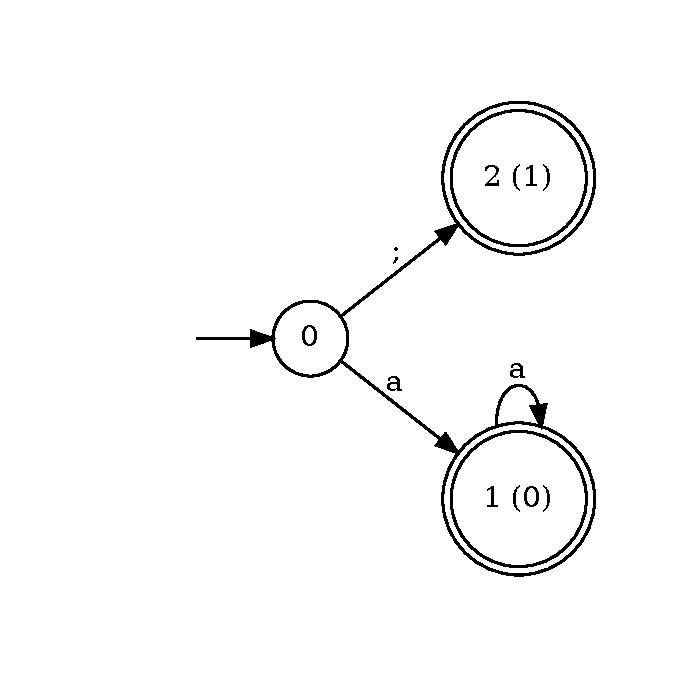
\includegraphics[width=\linewidth]{figures/certificate_sound.pdf}\\[0.5em]
(a) $a^+$ and \code{;}
\end{minipage}
\hfill
\begin{minipage}[b]{0.24\linewidth}
\centering
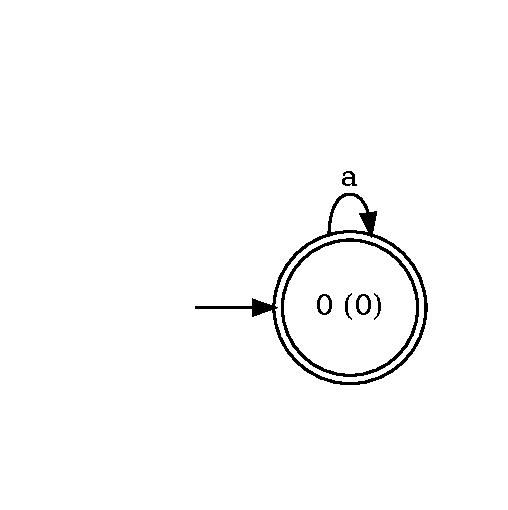
\includegraphics[width=\linewidth]{figures/certificate_nullable.pdf}\\[0.5em]
(b) $a^*$
\end{minipage}
\hfill
\begin{minipage}[b]{0.3\linewidth}
\centering
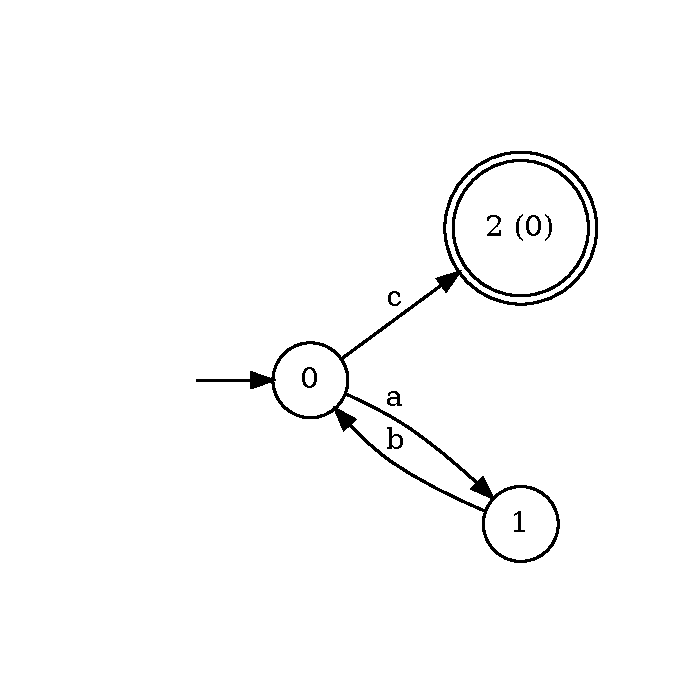
\includegraphics[width=\linewidth]{figures/certificate_cyclic.pdf}\\[0.5em]
(c) $(ab)^*c$
\end{minipage}
\caption{Minimized automata drawn by the library described here; double circles are accepting states,
labelled with the state number and the token identifier. In (a) nothing enters state 0, so \code{;} is certified: no
other state consumes it. In (b) state 0 accepts and re-enters itself on $a$, and in (c) it is re-entered through the
cycle $a, b$. In both counterexamples the only state consuming the candidate byte is the initial one, so dropping the
re-entrancy condition would certify it and break longest match. The shipped predicate rejects the candidate in (b) and
(c) and accepts \code{;} in (a).}
\label{fig:reentrancy}
\end{figure}

\section{Deriving and using the certificate}
\label{sec:derivation}

The certificate is derived by a linear-time analysis of the compiled transition table at construction time. First a
reverse pass computes $Q^+$: the table is inverted into a predecessor list, the accepting states seed a worklist, and
each state that reaches one is marked. A forward pass from $q_0$ then marks the reachable states, so that the two
together give the trim subautomaton the results are stated over; subset construction emits only reachable states, but
the analysis is exposed on a simulator that accepts any transition table, and an unreachable state left by a
hand-assembled one would otherwise produce false negatives. One scan then detects whether any reachable entry targets
$q_0$, establishing re-entrancy, and a sweep over the $|\Sigma| \times |Q|$ table records, for each byte, whether any
non-exempt reachable live state consumes it into $Q^+$. The result is a $|\Sigma|$-bit set. Every pass visits each
table entry a constant number of times, so the cost stays $O(|Q|\,|\Sigma|)$, with the same bound in auxiliary space
for the predecessor list; it is paid once, amortized into a construction that already did strictly more work to
produce the table, and the scanner's inner loop is untouched.

Three operations expose the property. A predicate reports whether a byte is a useful certified split symbol, the set of
Corollary~\ref{cor:useful}. A planner divides an input into chunks by sliding each interior boundary forward from its
equal-division target to the next certified byte, and returns a single chunk spanning the whole input when that useful
set is empty. An executor runs the plan, one thread per chunk, and by Theorem~\ref{thm:main} the concatenated per-chunk
streams equal the serial stream for completely tokenizable input, with Corollary~\ref{cor:malformed} governing the rest.
There is no speculation to retry, no overlap to verify, and no merge beyond concatenation.

For $k$ requested chunks the planner performs at most $k-1$ forward searches, so its worst case is $O(kN)$ over an input
of $N$ bytes when certified occurrences are rare; $k$ is normally a small hardware-thread count, and the searches start
at equally spaced offsets. A one-pass planner would reduce the worst case to $O(N + k)$. Section~\ref{sec:planning}
measures the range.

\begin{figure}[t]
\centering
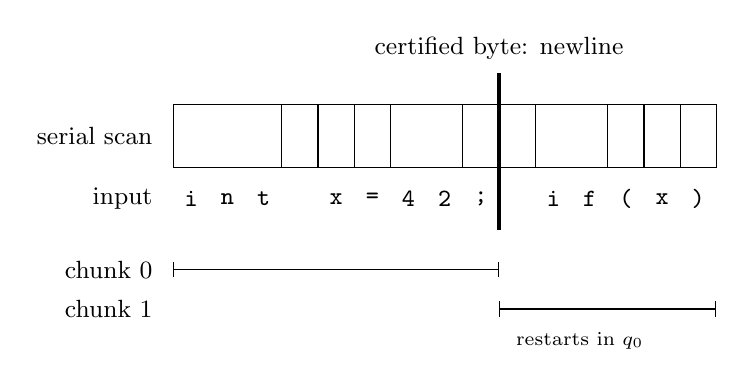
\begin{tikzpicture}[x=4.6mm, y=1mm, font=\small]
  % One cell per input byte, so the token boxes and the input line up exactly.
  % i n t _ x = 4 2 ; \n i f ( x )
  %  0 1 2 3 4 5 6 7 8  9 10 11 12 13 14
  \node[anchor=east] at (-0.3, 13) {serial scan};
  \node[anchor=east] at (-0.3, 5) {input};

  % token extents, as outlined boxes
  \foreach \s/\e in {0/2, 3/3, 4/4, 5/5, 6/7, 8/8, 9/9, 10/11, 12/12, 13/13, 14/14} {
    \draw (\s, 9) rectangle (\e + 1, 17);
  }

  % the input bytes, one per cell
  \foreach \i/\c in {0/i, 1/n, 2/t, 4/x, 5/=, 6/4, 7/2, 8/;, 10/i, 11/f, 12/(, 13/x, 14/)} {
    \node at (\i + 0.5, 5) {\ttfamily \c};
  }

  % the certified byte, and the boundary immediately before it
  \draw[very thick] (9, 1) -- (9, 21);
  \node[anchor=south] at (9, 21.5) {certified byte: newline};
  % the two chunks
  \node[anchor=east] at (-0.3, -4) {chunk 0};
  \draw[|-|] (0, -4) -- (9, -4);
  \node[anchor=east] at (-0.3, -9) {chunk 1};
  \draw[|-|] (9, -9) -- (15, -9);
  \node[anchor=west] at (9.2, -13) {\scriptsize restarts in $q_0$};
\end{tikzpicture}
\caption{A certified byte is a point where the serial scan is provably between tokens: no state reachable mid-token
consumes it into a state that can still accept, so the scan has finished a token and returned to $q_0$ exactly
there. A chunk may therefore start at
that offset with no entry-state uncertainty, and the two chunks' token streams concatenate to the serial one.}
\label{fig:split}
\end{figure}

\section{Applicability}
\label{sec:applicability}

The certificate asks the grammar for cooperation, and the interesting question is how much real token sets give.
Table~\ref{tab:applicability} was produced by compiling each token set and reading the predicate for all 256 byte
values. The predicate implements Corollary~\ref{cor:useful}, so it excludes the vacuous certificates of
Proposition~\ref{prop:vacuous} already and the column needs no further filtering. Rows two through four each add a
single token kind to the grammar of row one rather than accumulating, so each collapse is attributable to the token kind
named; the conventional and split-friendly rows recognize exactly the same byte language and differ only in the
tokenization, and the block-comment row directly after them adds one token kind to the split-friendly grammar, so those
three are read together. The program that produces the table
is \code{figures/applicability.cpp}, archived with this report; it links the library and asserts every row.

\begin{table}[t]
\centering
\begin{tabular}{p{8.4cm}p{5.4cm}}
\toprule
Token set & Useful certified bytes \\
\midrule
C-like: identifiers, numbers, whitespace runs, operators, punctuation & all operator and punctuation bytes \\
the first row plus string literals alone (no raw newline inside) & none \\
the first row plus \code{//} line comments alone & none \\
the first row plus block comments alone & none \\
JSON, the RFC 8259 lexical forms over bytes & none \\
log lines: a run of non-newline bytes, and newline & newline \\
C-like, conventional tokenization: line-bounded strings and \code{//} comments, whitespace runs including newline
& none \\
the same recognized language, split-friendly: newline its own token, spaces and tabs a separate run & newline \\
the same plus block comments & none \\
\code{keyword\_scale\_builder()}, the construction-cost grammar & 16 of those 24 bytes \\
\code{build\_lexer(false)}, the scaling grammar & 13 of its own 14 \\
\bottomrule
\end{tabular}
\caption{Certified bytes by token set. Three mechanisms explain the collapses: free-content tokens absorb the
alphabet, run-style trivia de-certifies its own bytes, and a multi-byte token de-certifies the bytes it continues past.}
\label{tab:applicability}
\end{table}

Three mechanisms explain the collapses. First, \emph{free-content tokens absorb the alphabet}: a string literal that may
contain \code{(} makes \code{(} a mid-token byte and de-certifies it everywhere, so one token kind with a near-total
interior alphabet removes almost every candidate. Second, \emph{run tokens de-certify their own bytes}: with whitespace
tokenized as a run over space, tab, and newline, the second newline of a blank line is consumed by the run's
continuation state, so newline itself becomes mid-token-consumable. The byte's own token kills it, which is easy to
miss.

Third, and in the same family, \emph{a multi-byte token de-certifies every byte that can follow its first}. The
survey's first row spells each operator as a single byte, so each is consumed only at the initial state and all
twenty-four certify. Section~\ref{sec:evaluation} measures two different C-like grammars, and the last two rows of
Table~\ref{tab:applicability} name them rather than describing them, since they disagree. The construction-cost
grammar, \code{keyword\_scale\_builder()} in \code{tools/benchmark/src/main.cpp}, spells operators as literals
including \code{++}, \code{==} and \code{->} and admits a decimal point inside a number. Every byte occurring after
the first position of some operator therefore has a live mid-token state on it, and seven candidates fall that way:
\code{= < > \& | + -}. The decimal point falls independently, not as an operator continuation but because
\code{decimal\_float()} admits it inside a number, bringing the total to eight. The scaling grammar,
\code{build\_lexer(false)} in \code{tools/benchmark/src/harness.cpp}, has a smaller operator set in which every
multi-byte operator has \code{=} as its only continuation byte, so only \code{=} is lost and thirteen of its fourteen
candidates certify. Both collapses are partial. What they show is that ``operators certify'' is a claim about the
particular literals a grammar registers, so the grammar has to be named rather than described: these two C-like
benchmark grammars recognize different operator and number languages, and they certify different sets. The sharper
claim, that certification depends on the tokenization and not on the recognized language, needs a pair recognizing the
same language, and the conventional and split-friendly rows below are that pair: identical token kinds and identical
accepted input, differing only in whether newline is folded into the whitespace run, and certifying nothing versus
certifying newline.

All three mechanisms point at the same design lever: certification is a property of the \emph{tokenization} rather
than an intrinsic one, and a tokenization can sometimes be refactored without changing what is recognized at all. The
split-friendly row
of Table~\ref{tab:applicability} keeps the identical C-like language but tokenizes newline as its own single-byte token,
leaves spaces and tabs as whitespace runs, and keeps strings and line comments line-bounded. The row directly above it
is the same language under the conventional tokenization and certifies nothing, which isolates the change. Then newline
certifies, and
the folklore rule follows as a practical corollary: for conventional tokenizations in which newline is its own token,
line-based splitting is sound when no other token can contain a newline. The automaton-level statement remains the exact
one; ``no token spans a line'' is sufficient here but not necessary in general, since a token that merely \emph{begins}
with newline leaves the certificate intact. Adding block comments, the one token kind in the surveyed split-friendly
tokenization that spans lines, destroys the certificate again, which is the formal shape of both ``you cannot chunk C by
lines'' and the quoted-newline problem that pushed CSV parsing into speculation.

The JSON row of Table~\ref{tab:applicability} appears to contradict the literature, and the reconciliation is about the
equivalence each result preserves rather than about the automaton. Prior claims that JSON may be divided at
newline~\cite{barenghi2015parallel,li2021plex} treat whitespace as unobservable trivia. Such a division can split one
maximal whitespace match into two ignored matches whose lengths sum to the original, leaving the observable non-trivia
stream unchanged. Theorem~\ref{thm:main} preserves something stronger, the complete sequence of emitted kinds and
lengths, and under that semantics a newline inside a maximal whitespace token is not a certified boundary. The grammar
surveyed here follows the RFC 8259 lexical forms~\cite{bray2017json} over byte input, with the full string escapes,
signed numbers with fraction and exponent, the three literal names, and whitespace runs emitted as tokens, so it is
refused exactly as it should be. It is a lexer over bytes rather than a conforming JSON processor: string interiors
admit any byte from \code{0x20} up except quote and backslash, so UTF-8 well-formedness, which RFC 8259 requires of
JSON exchanged outside a closed ecosystem, is
assumed of the input rather than checked here. That is orthogonal to certification, since validating it would only
remove bytes from string interiors and so could not de-certify anything that certifies now. The two results do not
conflict; they quantify over different streams. A scanner that discards trivia can therefore split safely at newline
under the weaker observable-stream equivalence, but Definition~\ref{def:certified} still rejects newline: the whitespace
continuation state consumes it either way. Recovering certification itself needs the tokenization changed, for instance
by making newline its own token as in the split-friendly row above, or the theorem extended to reason modulo ignored
kinds.

\section{Evaluation}
\label{sec:evaluation}

The evaluation reports two machines. The first is the one the method was developed on and is retained because the
contrast with the second is itself a result: a figure that looks like a property of the API on one does not hold its
value, or even its sign, across environments and benchmark revisions.

\paragraph{Environment A, virtualized.} An Intel Core i9-12900K, a hybrid part with eight performance cores carrying
two-way SMT and eight efficiency cores, so sixteen physical cores and 24 logical processors, on an ASUS ROG Maximus
Z690 Hero with 32\,GiB of memory. The host is Windows 11 build 26200 with virtualization-based security enabled;
the measurements ran under WSL 2.7.11 on kernel 6.18.33.2-microsoft-standard-WSL2, Ubuntu 24.04.4 LTS, glibc 2.39,
with all 24 logical processors and 15\,GiB of memory visible to the guest. Compiled by GCC 13.3.0 at \code{-O2}.
Corpora are 16\,MiB and fixed-seed, scenarios run in a fixed order, and the archive holds summaries only
(\code{data/benchmark.txt}).

Four properties of this environment bound what its figures establish, and we state them rather than adjust for them.
The guest does not see the host's hybrid topology: it reports twelve cores of two threads each, so a performance core
is indistinguishable from an efficiency core from inside the measurement. Threads are not pinned, and could not
usefully be while that holds. The guest is given no \code{cpufreq} interface, so the clock is neither fixed nor
observable. And the machine was not quiesced. The corpora are also cache-resident, 16\,MiB against a 30\,MB
last-level cache, so these are warm-cache figures throughout.

\paragraph{Environment B, bare metal.} An AMD Ryzen 9 9950X3D, sixteen physical cores with two-way SMT across two L3
domains of eight cores each, 128\,MiB of L3 in total, 59\,GiB of memory, Ubuntu 26.04 on kernel 7.0.0-28-generic,
compiled by GCC 15.2.0 at \code{-O2}. The \code{performance} governor was set, which biases the clock toward its
maximum but does not fix it: boost remains enabled, and the archived \code{lscpu -e} of the pinned run reported in
Table~\ref{tab:scaling} shows 22 distinct frequencies between 624 and 5711\,MHz across the 32 processors at the
instant it was taken. The clock is therefore observable
here, unlike in Environment A, but not controlled. The topology is visible and archived; scenarios run in interleaved
rounds reshuffled per round from a fixed seed; and corpora sweep 1, 16, 128 and 512\,MiB. Every pass of the ten
scaling scenarios is recorded individually in \code{data/bare-metal-unpinned-run2/} and
\code{data/bare-metal-pinned-run2/}; the construction, planning and thread-launch figures below are summaries over 15
passes, not per-pass records.

This environment is measured in two placements, each run twice, giving four archives. The unpinned runs may place
threads on any of the 32 logical processors. The
pinned run confines the process to the eight physical cores of a single L3 domain (\code{taskset -c 0-7}), which
excludes the SMT siblings and the other L3 domain from the set the scheduler may use, so eight threads have eight
distinct physical cores available to them. It constrains placement rather than fixing it: threads remain free to
migrate within those eight cores, and nothing prevents two from sharing one. It
was not quiesced either: three login sessions were present, with load averages of 0.55 and 1.83 before the unpinned
and pinned runs of Tables~\ref{tab:scaling} and~\ref{tab:planning}. The second figure is largely the first run's own
residue, the two having started two minutes apart, which is itself the point: the machine was busy with the previous
measurement.

The 512\,MiB corpus is four times the machine's aggregate last-level cache, and the pinned process is confined to
one of the two L3 domains, so it exceeds whatever share is actually reachable by a comfortable margin. The archive
does not record the two domains' capacities separately, so the sweep is read conservatively: 512\,MiB is out of cache
under any split of the 128\,MiB aggregate.
Before any timing, and in both environments, the benchmark checks that the chunked token stream is identical to the
serial one by an exact (kind, length) comparison.

\subsection{Scaling}

Table~\ref{tab:scaling} reports median throughput on Environment B, pinned, which is the most constrained
configuration measured:
visible topology, eight physical CPUs of one L3 domain with the SMT siblings excluded, a clock biased to maximum, and
a corpus sweep that leaves the cache. Two baselines matter, they answer different questions, and only one of them turns
out to hold still between collections. The parallelism itself is measured against the same API driven with a single
chunk, which
plans, uses the per-chunk sink, and spawns nothing: against it the certified splitting reaches $1.96\times$,
$3.87\times$, and $7.63\times$ on the 512\,MiB dense corpus, or 98\%, 97\% and 95\% parallel efficiency; the other
collection of the same placement gives 95\%, 93\% and 93\%. A user
choosing between the serial and parallel entry points compares instead against the plain scan, and gains
$3.46\times$ at four chunks in this collection and $3.94\times$ in the other collection with the same placement.
Conflating the two,
as an end-to-end table alone would, charges parallelization for the sink and inherits an unstable denominator.

\begin{table}[t]
\centering
\begin{tabular}{lrrrrrr}
\toprule
Corpus & size & plain scan & 1 chunk & 2 chunks & 4 chunks & 8 chunks \\
\midrule
dense (1.83 B/token)  & 1\,MiB    & 767.5 & 728.5 & 1436.1 & 2780.4 & 4685.9 \\
                      & 16\,MiB   & 771.5 & 686.9 & 1374.3 & 2679.5 & 5074.6 \\
                      & 128\,MiB  & 788.4 & 722.8 & 1432.1 & 2782.3 & 5420.4 \\
                      & 512\,MiB  & 818.0 & 730.1 & 1434.2 & 2828.0 & 5568.3 \\
\midrule
source (3.53 B/token) & 512\,MiB  & 757.5 & 711.1 & 1415.0 & 2763.0 & 5500.5 \\
\bottomrule
\end{tabular}
\caption{Median throughput in MiB/s on Environment B with the process pinned to one L3 domain, second run. The
one-chunk column is the parallel API without parallelism, and is the baseline the parallel efficiencies use; the
plain-scan column does not hold still between collections and is discussed below.}
\label{tab:scaling}
\end{table}

Scaling does not depend on the corpus fitting in cache. The 512\,MiB corpus is four times the machine's 128\,MiB of
last-level cache, and its eight-chunk efficiency, 95.3\%, is the highest of the four sizes rather than the lowest: the
figures are 80.4\%, 92.3\%, 93.7\% and 95.3\% at 1, 16, 128 and 512\,MiB, so efficiency rises with input size and
keeps rising across the cache boundary rather than stepping down at it. The sweep does not locate a break-even input
size, because it never reaches one: even at the smallest size measured, eight chunks are $6.43\times$ the one-chunk
API. What it shows is where fixed overhead becomes visible, at 1\,MiB, where efficiency falls to 80.4\% because
spawning and joining eight threads costs about 40\,$\mu$s against a scan of roughly 1.4\,ms.

\paragraph{What placement costs.} Running the same measurement unpinned, free to use all 32 logical processors, lowers
eight-chunk efficiency from 95\% to 93\% at 512\,MiB and from 80\% to 68\% at 1\,MiB, the gap falling from twelve
points at 1\,MiB to about three at 512. The two- and four-chunk figures move by two points or less at 128 and 512\,MiB
and by more at the smaller sizes. One hypothesis is SMT: with eight threads free on 32 logical processors, some pairs
share a physical core. We do not claim it, and cannot from this data. For each benchmark revision there is one run per
placement, taken at different times rather than as replicated interleaved conditions, and a gap also appears at two
chunks where collisions should be rare. Attributing it would need paired repeated runs, or per-thread CPU residence
recorded during the scan. What the two runs support is narrower: on these runs the restricted CPU set performed better
at eight chunks, and certified splitting delivered most of its benefit in both.

\paragraph{The two collections are not a controlled repeat.} Environment B was collected twice in each placement, but
the two collections were taken at different commits: between them the benchmark began writing round-trip-safe CSV
values and gained the four plan-and-execute scenarios that now run before the scaling sweep. The scaling code itself is
unchanged, but the executable, its layout, and what executes before the measurement are not. These are therefore two
benchmark revisions on one machine rather than repeated runs of one experiment, and the difference between them cannot
be attributed to the machine.

The largest differences are in the single-threaded rows, and their direction is the same under both placements. At
512\,MiB on the dense corpus the plain scan rose 14.3\% pinned and 17.4\% unpinned, while the one-chunk row fell
3.7\% and 3.8\% respectively. At that size the multi-chunk rows move much less: at most 0.8\% on the dense corpus
pinned and 1.4\% on the source corpus, 1.1\% and 0.6\% unpinned. That stability is specific to 512\,MiB and does
not hold across the sweep, where multi-chunk rows move by as much as 5.9\% pinned and 6.3\% unpinned, both at
16\,MiB. A single-threaded shift that lands within 0.1 points under two different affinities looks more like a
property of the revision than of the scheduler, though nothing here isolates which.

The comparison between the plain scan and the one-chunk row is the quantity this moves. It has now taken three values:
14\% \emph{below} on Environment A, 5.9\% \emph{above} in the first Environment B collection at 512\,MiB, winning 13 of
15 same-round pairs, and 10.7\% below in the second, reported in Table~\ref{tab:scaling}, winning none of 15. We report
that rather than explain it. The consequence for the figures above is that efficiencies measured against the one-chunk
baseline moved by two to four points between the collections, 93\% to 95\% at eight chunks, while the end-to-end ratio,
which divides by the plain scan, moved by 12\%. That is why the first is quoted as a range of a few points and the
second as a range of nearly half a turn.

\subsection{Planning cost}
\label{sec:planning}

Table~\ref{tab:planning} measures the planner alone, over a 16\,MiB input divided into eight chunks, as certified bytes
grow scarce. The certified byte is newline; the inputs place newlines every 40 bytes, every 1\,MiB, and never, and the
last row uses a token set that certifies nothing at all. Scarcity is not a contrived case: machine-generated JSON often
carries no newlines at all, which both prior works give as a reason to distrust delimiter
splitting~\cite{barenghi2015parallel,li2021plex}.

\begin{table}[t]
\centering
\begin{tabular}{lrrr}
\toprule
Certificate density & chunks planned & median & bytes scanned \\
\midrule
newline every 40 bytes    & 8 & 0.1\,$\mu$s     & $<$ 1\,KiB \\
newline every 1\,MiB      & 8 & 1021.0\,$\mu$s  & 3.5\,MiB \\
certified byte absent     & 1 & 16365.5\,$\mu$s & 56\,MiB \\
nothing certified         & 1 & 0.0\,$\mu$s     & 0 \\
\bottomrule
\end{tabular}
\caption{Boundary planning for $k=8$ over 16\,MiB on Environment B, pinned. The two scanning rows show similar
effective scan rates, 3.35 and 3.34\,GiB/s, consistent with the $O(kN)$ bound; the last row is the empty-certificate
fast path. Each pass repeats
the plan until the sample outlasts the clock, so the sub-microsecond rows measure planning rather than timer
resolution.}
\label{tab:planning}
\end{table}

The two middle rows cross-check each other: 3.5\,MiB scanned in 1.02\,ms and 56\,MiB in 16.4\,ms give similar effective
scan rates, which is consistent with the $O(kN)$ bound and indicates that the planner's cost is dominated by the forward
searches rather than by anything else it does. Even its worst case, a certificate whose byte never occurs in a 16\,MiB
input, costs 16.4\,ms once; a caller planning a much smaller chunk count, or planning once and scanning repeatedly,
pays proportionally less. The empty-certificate case is answered
without touching the input.

That worst case is a cost the caller pays before any scanning begins, and on such an input the planner returns a
single chunk, so the scan that follows is the serial one. Stating it end to end needs planning and scanning timed on
one grammar over one input, which the earlier planning rows do not provide: they use a two-token grammar over a
synthetic input while the scaling rows use the C-like grammar over generated source, and adding those would compare
different lexers over different inputs. A separate scenario therefore times both phases together on the planning
workload. With the certified byte absent, the parallel entry point takes 34.5\,ms against 18.2\,ms for the serial
one, so choosing it costs $1.90\times$; with certified bytes every 40 bytes it takes 1.7\,ms against 12.4\,ms, a
gain of $7.3\times$. Both emit 838861 tokens, or one, identically. The penalty is a property of the planner as
implemented, not of the certificate. The planner here is deliberately simple, one forward search per boundary, and
the one-pass $O(N + k)$ formulation above reduces that worst case to a single pass over the input, under 5\,ms
here, rather than eliminating it; the distinction it draws attention to is that
\emph{deciding} the certificate needs no input at all, while \emph{locating} its occurrences is a runtime scan whose
cost depends on how often the byte actually appears.

\subsection{Correctness}

Three levels of evidence support the implementation. The benchmark compares the chunked and serial token streams exactly
before timing. The unit suite carries the counterexamples of Section~\ref{sec:subtlety}, including the nullable and
cyclic re-entry cases. A fuzzer generates arbitrary token sets and inputs, checks every planned boundary against the
predicate, and compares the concatenated parallel stream against the serial one on every execution; local extended
fuzzing and a bounded fuzzing job on every continuous integration run have found no violation.

\section{Limitations and future work}

The result is scoped to one fixed token automaton restarting from one fixed initial state. A scanner carrying state the
automaton does not represent falls outside it: lexer modes, indentation stacks, semantic predicates, and hand-written
scanning for constructs the regular grammar cannot express all carry information across token boundaries, and such state
must either be folded into the automaton or treated as a region boundary the plan does not cross. The theorem also
preserves the token \emph{sequence} and nothing more; a caller whose sink has externally visible side effects still
needs its own ordering, since chunks run concurrently and only the concatenation is specified.

The approach trades generality for certainty. When the grammar does not cooperate it offers no usable split points, by
design, and the composition and speculation families of Section~\ref{sec:prior} remain the only options. Several
extensions look natural. A \emph{conditional} certificate over symbol pairs or short windows, for instance ``\code{)}
followed by newline'', would recover splitting for grammars where no single byte certifies. A hybrid plan could split at
certified bytes where they exist and fall back to speculative entry elsewhere, keeping the guarantee where it is free
and paying for it only where it is not. The grammar-refactoring lever of Section~\ref{sec:applicability} could be
automated: given a token set, propose the minimal trivia re-tokenization that makes a chosen byte certify. The
certificate is also orthogonal to a separate cost of longest-match scanning: after a failed longer match the scan
resumes at the last accepting position, so a token set whose long patterns repeatedly fail back to short ones is
quadratic in the input, and splitting into chunks reduces the constant without changing the shape. The quadratic
pathology can be removed with per-position information, obtained either during the scan or before it: Reps keeps the
backtracking loop but tabulates the state and position pairs that have already failed, so no doomed transition is
repeated~\cite{reps1998maximal}, while the uniform-tokenization algorithms precompute what each suffix admits in an
initial right-to-left pass~\cite{li2025uniform}. Finally, the evaluation rests on two x86-64 machines,
one Alder Lake under virtualization and one Zen 5 on bare metal, with threads constrained only to a CPU set rather
than pinned individually; a non-x86 architecture, and per-thread placement, would strengthen the scaling claims,
though not the correctness ones.

\section{Related work}

A certified split symbol is not a synchronizing word in the classical sense~\cite{volkov2008synchronizing}. A
synchronizing word maps \emph{every} state to one common state; a certified symbol is one that no reachable mid-token
state may consume into a state that can still accept, so the surrounding longest-match loop must already have finished
its token and returned to $q_0$ before the symbol arrives. The reset comes from the token loop, not from the transition
structure.

Certified split points differ from simultaneous automata in requiring no enlarged automaton and no composition, from
speculation in requiring no guess and no repair, from $k$-locality in being a per-symbol property derived from the token
loop's reset rather than a uniform property of the automaton, from realignment after the fact in merging nothing, and
from
delimiter folklore in deriving the safe set from the compiled token set rather than assuming it per format. The
derivation also correctly refuses the grammars for which the folklore is unsound. The contribution is therefore narrow
and specific. Relocating cuts to a separator is classical, and the observation that it works for JSON but needs Lua's
grammar constrained first is stated in the literature; what appears to be missing is the automatic certification step
those choices leave implicit, namely a sound grammar-only test of whether a given byte is a safe separator for a given
token set. The certificate supplies that test from the compiled automaton, with no hand analysis and no
input-dependent context-recovery pass, and the survey of Section~\ref{sec:applicability} turns the same machinery into
a statement about which token sets admit such bytes at all. The analysis is not merely sound.
Theorem~\ref{thm:necessity} shows the condition is also necessary once the analysis is restricted to $A^+$, which is
what the derivation of Section~\ref{sec:necessity} does, so on a compiled token set the test rejects a byte exactly
when a witness input exists that places it inside a token. That matters for reading Section~\ref{sec:applicability}: a
row saying nothing certifies is a fact about the tokenization, not a limit of the analysis.

We are not aware of prior work stating this condition, in particular the re-entrancy requirement, as a static per-symbol
property of the token DFA, though its components are all classical. We checked that claim against the parallel lexing
and parallel finite-automata literature, the theory of synchronizing automata, incremental lexical analysis, and the
recent work on sequential~\cite{reps1998maximal,li2025uniform} and streaming~\cite{li2026streaming} tokenization. Each
answers a neighbouring question: where to restart after an edit, how to reset every state at once, how to avoid
repeated rescanning, how to recover a chunk's entry state after the fact~\cite{voetter2021gpu}. None asks which
single bytes the token set makes safe in advance.

\section{Conclusion}

A byte is a certified split symbol of a compiled token set when, among the transitions that can still end in acceptance,
no state but the initial one consumes it, and, if the initial state consumes it, that state is not re-entrant. Every
occurrence of such a byte in a completely tokenizable input begins a token, so chunk boundaries placed there preserve
the token stream exactly, with no speculation, no overlap, and no merge beyond ordered concatenation. The re-entrancy
clause is what makes this true rather than nearly true: without it the natural incoming-transition criterion certifies
$a$ for the token set $a^*$ and splits $aa$ into two tokens where the scanner yields one.

The condition is necessary as well as sufficient once the analysis is restricted to states from which acceptance is
still reachable, so a token set with no certified byte has no single-byte split symbol at all, rather than merely
defeating the test. Deriving the certificate is a linear-time sweep of the transition table at construction time, and
the same sweep decides which certified bytes can occur in valid input at all. That makes the applicability question
mechanical, and the answer is often negative: a single token kind with a near-total interior alphabet, such as a block
comment, removes every useful certificate from an otherwise cooperative C-like grammar. Where the certificate is
non-empty the measured gain is 93--95\% parallel efficiency at eight threads against the same API driven with one
chunk, on a 512\,MiB corpus that does not fit in cache, and $3.5$--$3.9\times$ end to end at four threads. Both are
ranges across two benchmark revisions on one machine. The wider end-to-end range comes from the serial baseline used
as its denominator: at 512\,MiB the multi-chunk rows move far less between the revisions than that baseline does;
Section~\ref{sec:evaluation} reports that separately.

The contribution is therefore narrow and exactly bounded: not another way to lex in parallel, but the automaton-derived
certification step that prior delimiter-based systems have handled through language-specific reasoning.

\bibliographystyle{plain}
\bibliography{refs}

\end{document}
